% !TeX encoding = UTF-8
% !TeX spellcheck = en_US

\documentclass[
	accentcolor=tud1a %Pick the color
]{tudreport}

% A couple of packages that may be useful
\usepackage{amsmath}
\usepackage{amsfonts}
\usepackage{amsthm}
\usepackage{algorithm2e}
\usepackage{listings}
\usepackage{xcolor}
\usepackage{tikz}
\usepackage{booktabs}
\usepackage{subfigure}
\usepackage[english]{babel}
\usepackage{blindtext}

% Defining JavaScript listings
\definecolor{mygreen}{rgb}{0,0.3,0}
\definecolor{myyellow}{rgb}{0.3,0.3,0}
\definecolor{mygrey}{rgb}{0.9,0.9,0.9}

\lstdefinelanguage{JavaScript}{
  keywords={break, case, catch, continue, debugger, default, delete, do, else, false, finally, for, function, if, in, instanceof, new, null, return, switch, this, throw, true, try, typeof, var, void, while, with},
  morecomment=[l]{//},
  morecomment=[s]{/*}{*/},
  morestring=[b]',
  morestring=[b]",
  ndkeywords={class, export, boolean, throw, implements, import, this},
  keywordstyle=\color{blue}\bfseries,
  ndkeywordstyle=\color{darkgray}\bfseries,
  identifierstyle=\color{black},
  commentstyle=\color{purple}\ttfamily,
  stringstyle=\color{red}\ttfamily,
  sensitive=true
}

\lstset{
    frameround=fttt,
    language=JavaScript,
    numbers=left,
    breaklines=true,
    breakatwhitespace=true,
    keywordstyle=\color{blue}\bfseries, 
    basicstyle=\ttfamily\color{black},
    numberstyle=\color{black},
    stringstyle=\color{myyellow},
    commentstyle=\color{mygreen},
    backgroundcolor=\color{mygrey}
    }
\lstMakeShortInline[columns=fixed]|

%\begin{lstlisting}[float,caption=Code Example,label=l:code_example]
%var a;
%console.log(a);
%if(a) {
%	// This is a comment
%	console.log('Yeah');
%}
%\end{lstlisting}

\begin{document}
\title{ARSE: Agile Responsive Simple Environment}
\subtitle{Team Echo: Project Report for the course Internet Praktikum TK in WS 2015/16}
\subsubtitle{Elmi Faisal Ali \\
Enkhtuul Gankhuyag \\
Floriment Klinaku \\
Masaud Yakubu Alhassan \\
Omar Antonio Erminy Ugueto \\
Satia Herfert
}

\maketitle

\tableofcontents

\chapter{Introduction}
\label{ch:introduction}

\blindtext

\chapter{Architecture}
\label{ch:architecture}

\chapter{User Documentation}
\label{ch:use-documentation}

In this chapter we will roughly explain how to use our application. For each state or thematic group of our application, there is a section that explains the graphical layout and the possible ways to interact with the application.

%TODO include the last tasks (like chat) somewhere.

%TODO cut the browser part of the screenshots
%TODO augment the screenshots with numbers/text etc., and refer to these numbers in the explanatory text.

\section{Profile Management}
\label{sec:profile-mgmt}
%Explain: Register, Login, Logout, change Profile

\begin{figure}
	\centering
	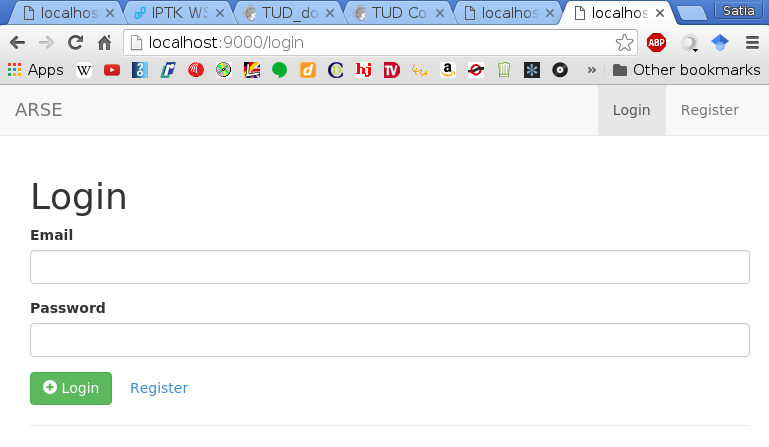
\includegraphics[width=0.5\textwidth]{img/login}
	\caption{The login screen.}
	\label{fig:login}
\end{figure}

When first visiting the ARSE app, you will be asked to login or register. The screen you will see is displayed in figure \ref{fig:login}. Here you can pass the form to login or click \emph{Register} to switch to a different form, where you are asked to register providing your full name, email address and a password. Email addresses serve as usernames and must be unique in the system.

After logging in, you can click your name in the upper right corner to access a page that allows to edit your profile. In that page you can adjust your name and password, but not your email address. The email address cannot be changed after the registration. Changes to your profile always require a password confirmation using your current password.

In the upper right corner you will also find a button that logs you out from the system.

\section{Project Management}
\label{sec:project-mgmt}
%Explain: List of projects, create project, modify/delete project.

After logging in, you will be redirected to a page that shows the projects you are a member of. If you just registered, this page will be empty. You can now create your own projects or ask colleagues to add you to their projects.

In order to create a project, click the button \emph{Create a new project}. This will open a form where you need to fill out name and description of the project. After that, the project will appear in the list and you will automatically become product owner of this project. This gives you privileges that normal developers in a project do not have.

The projects are listed with name and description. If you are product owner of a project, buttons are present, that you can use to delete or modify a project.

\begin{figure}
	\centering
	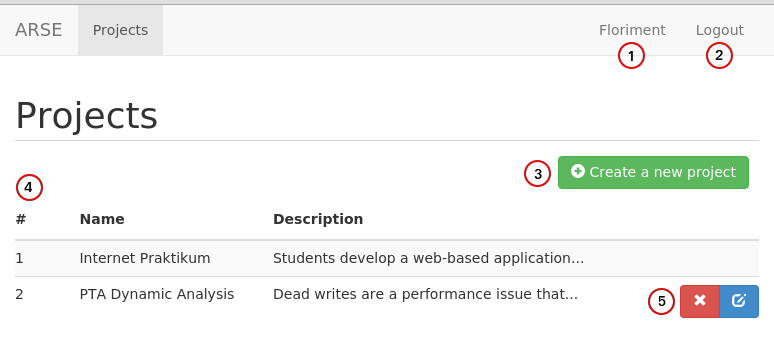
\includegraphics[width=0.5\textwidth]{img/projects}
	\caption{The project list screen.}
	\label{fig:project-list}
\end{figure}

%Explain: Project-navbar
You can click the name of a project in the list to access the project page. When you click it, you are redirected to a project specific are, which includes a navigation bar to access the different views available for each project. On the left-hand side of figure \ref{fig:project-backlog}, the project navigation bar is displayed. It includes five icons, and the views linked to them are listed in the following.
\begin{description}
	\item[Product Backlog:] A list of all stories of the project can be viewed here. Stories can be added, removed and edited. Furthermore, it is possible to start a new sprint in this view.
	\item[Sprint Board:] This view can only be accessed if a sprint is currently running. Its purpose is to allow changing the status of stories, managing the tasks of stories, or to close or cancel a sprint.
	\item[User management:] The participants of the project are displayed in this view. As a product owner, it is also possible to add or remove members, and to change their roles.
	\item[Past Sprints:] This view simply lists all finished sprints, with their time-frames and the number of story points that was burnt in the sprint.
	\item[Project configuration:] This view is only accessible by product owners and the icon will be hidden for developers. The view allows to define additional story types and statuses. These can then be used for every story of the project later on.
\end{description}


\subsection{Product Backlog}
\label{sec:backlog}

Explain: Adding items, viewing/modifying/deleting items, reordering items, dragging sprint delimiter, starting sprint.

\begin{figure}
	\centering
	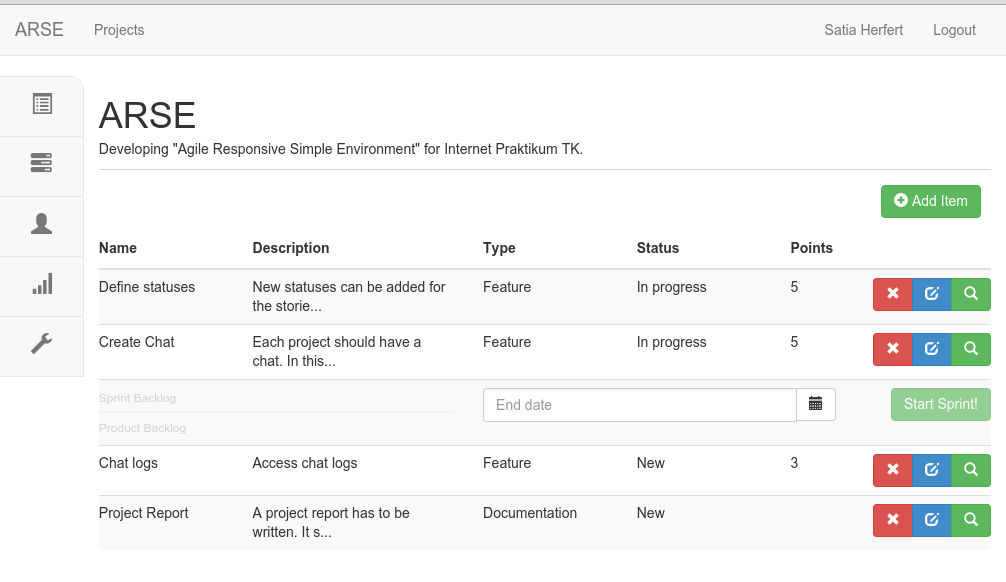
\includegraphics[width=0.5\textwidth]{img/backlog}
	\caption{The project backlog screen and the project navigation on the left-hand side.}
	\label{fig:project-backlog}
\end{figure}

\subsection{Sprint Board}
\label{sec:sprint-board}

Explain: Cancelling sprint, closing sprint, dragging stories, viewing stories, assigning a team member, adding tasks, changing tasks, dragging tasks, collapse/expand to view tasks.

\subsection{User Management}
\label{sec:user-mgmt}

Explain: List of members, assign role, remove members, add members with a certain role

\subsection{Project Configuration}
\label{sec:proj-config}

Explain: Adding story types, removing story types, adding statuses, removing statuses

\chapter{Done Product Backlog Items}
\label{ch:done-pbis}

In the following we list all the items from the original Product Backlog that were developed in this project. Certain stories have been moved to make the actions available to a different class of users, so that the product is more compatible with the idea of Scrum. The roles in our project are users, registered users, team members (of a project), and product owners (of a project). This list also contains stories that were modified or added to the original backlog.

%TODO go through our modified backlog and see if we need to add more stories here.

\begin{itemize}
	\item As a user, I can
	\begin{itemize}
		\item register to the system with user name, email and password. (Unique usernames)
		\begin{itemize}
			\item Users can be assigned to different projects with different roles.
		\end{itemize}
		\item access the web application with different kinds of devices (mobile, tablet, pc ...).
	\end{itemize}
	
	\item As a registered user, I can
	\begin{itemize}
		\item edit my profile (name, password).
		\item see the list of projects I am a member of.
		\item create new projects (name and description), and become automatically the product owner of these projects.
	\end{itemize}

	\item  As a team member of a project, I can
	\begin{itemize}
		\item access the Product Backlog
		\item access the Sprint Board
		\item access past Sprints which includes its name, time interval, and story points burnt.
		\item copy backlog items to the Sprint backlog.
		\item create new tasks in the task board (a task always belongs to a user story).
		\item change tasks including their description as well as their status (New, in progress, done).
		\item assign tasks to a team member.
		\item add new product backlog items to the product backlog of a project
		\begin{itemize}
			\item product backlog items can have different statuses (new, in progress, done).
			\item product backlog items can be of different types, e.g. feature, enhancement, fix
		\end{itemize}
		\item change the content of user stories
		\item change the order (priority) of user stories in the product backlog
		%\item chat with my team members
		%\item access and search chat logs
	\end{itemize}
	
	\item As a product owner of a project, I can
	\begin{itemize}
		\item create a new Sprint (a new Sprint cannot be created if there's one already running) with name, description, time-box and initial Sprint Backlog.
		\item assign registered users to a project.
		\item assign roles to project members (team member, product owner).
		\item change the list of statuses assignable to product backlog items in the project settings.
		\item change the list of types assignable to product backlog items in the project settings.
		\item close a Sprint (all done stories will be removed).
		\item cancel a Sprint
	\end{itemize}
\end{itemize}

%TODO Include a list of undone stories (if we have any)
%Bonus features
%users must confirm their registration by clicking on a registration link sent via email
%feature of burndown charts
%use special interaction features with mobile devices like shaking

\bibliographystyle{abbrvnat}
\bibliography{references}
\end{document}
